\documentclass[conference,compsoc]{IEEEtran}
 
\usepackage{datetime}

% *** CITATION PACKAGES ***
%
\ifCLASSOPTIONcompsoc
  % IEEE Computer Society needs nocompress option
  % requires cite.sty v4.0 or later (November 2003)
  \usepackage[nocompress]{cite}
\else
  % normal IEEE
  \usepackage{cite}
\fi
% cite.sty was written by Donald Arseneau
% V1.6 and later of IEEEtran pre-defines the format of the cite.sty package
% \cite{} output to follow that of the IEEE. Loading the cite package will
% result in citation numbers being automatically sorted and properly
% "compressed/ranged". e.g., [1], [9], [2], [7], [5], [6] without using
% cite.sty will become [1], [2], [5]--[7], [9] using cite.sty. cite.sty's
% \cite will automatically add leading space, if needed. Use cite.sty's
% noadjust option (cite.sty V3.8 and later) if you want to turn this off
% such as if a citation ever needs to be enclosed in parenthesis.
% cite.sty is already installed on most LaTeX systems. Be sure and use
% version 5.0 (2009-03-20) and later if using hyperref.sty.
% The latest version can be obtained at:
% http://www.ctan.org/pkg/cite
% The documentation is contained in the cite.sty file itself.
%
% Note that some packages require special options to format as the Computer
% Society requires. In particular, Computer Society  papers do not use
% compressed citation ranges as is done in typical IEEE papers
% (e.g., [1]-[4]). Instead, they list every citation separately in order
% (e.g., [1], [2], [3], [4]). To get the latter we need to load the cite
% package with the nocompress option which is supported by cite.sty v4.0
% and later.

% *** GRAPHICS RELATED PACKAGES ***
%
\ifCLASSINFOpdf
  % \usepackage[pdftex]{graphicx}
  % declare the path(s) where your graphic files are
  % \graphicspath{{../pdf/}{../jpeg/}}
  % and their extensions so you won't have to specify these with
  % every instance of \includegraphics
  % \DeclareGraphicsExtensions{.pdf,.jpeg,.png}
\else
  % or other class option (dvipsone, dvipdf, if not using dvips). graphicx
  % will default to the driver specified in the system graphics.cfg if no
  % driver is specified.
  % \usepackage[dvips]{graphicx}
  % declare the path(s) where your graphic files are
  % \graphicspath{{../eps/}}
  % and their extensions so you won't have to specify these with
  % every instance of \includegraphics
  % \DeclareGraphicsExtensions{.eps}
\fi
% graphicx was written by David Carlisle and Sebastian Rahtz. It is
% required if you want graphics, photos, etc. graphicx.sty is already
% installed on most LaTeX systems. The latest version and documentation
% can be obtained at: 
% http://www.ctan.org/pkg/graphicx
% Another good source of documentation is "Using Imported Graphics in
% LaTeX2e" by Keith Reckdahl which can be found at:
% http://www.ctan.org/pkg/epslatex
%
% latex, and pdflatex in dvi mode, support graphics in encapsulated
% postscript (.eps) format. pdflatex in pdf mode supports graphics
% in .pdf, .jpeg, .png and .mps (metapost) formats. Users should ensure
% that all non-photo figures use a vector format (.eps, .pdf, .mps) and
% not a bitmapped formats (.jpeg, .png). The IEEE frowns on bitmapped formats
% which can result in "jaggedy"/blurry rendering of lines and letters as
% well as large increases in file sizes.
%
% You can find documentation about the pdfTeX application at:
% http://www.tug.org/applications/pdftex


% *** MATH PACKAGES ***
%
%\usepackage{amsmath}
% A popular package from the American Mathematical Society that provides
% many useful and powerful commands for dealing with mathematics.
%
% Note that the amsmath package sets \interdisplaylinepenalty to 10000
% thus preventing page breaks from occurring within multiline equations. Use:
%\interdisplaylinepenalty=2500
% after loading amsmath to restore such page breaks as IEEEtran.cls normally
% does. amsmath.sty is already installed on most LaTeX systems. The latest
% version and documentation can be obtained at:
% http://www.ctan.org/pkg/amsmath

% *** SPECIALIZED LIST PACKAGES ***
%
%\usepackage{algorithmic}
% algorithmic.sty was written by Peter Williams and Rogerio Brito.
% This package provides an algorithmic environment fo describing algorithms.
% You can use the algorithmic environment in-text or within a figure
% environment to provide for a floating algorithm. Do NOT use the algorithm
% floating environment provided by algorithm.sty (by the same authors) or
% algorithm2e.sty (by Christophe Fiorio) as the IEEE does not use dedicated
% algorithm float types and packages that provide these will not provide
% correct IEEE style captions. The latest version and documentation of
% algorithmic.sty can be obtained at:
% http://www.ctan.org/pkg/algorithms
% Also of interest may be the (relatively newer and more customizable)
% algorithmicx.sty package by Szasz Janos:
% http://www.ctan.org/pkg/algorithmicx


% *** ALIGNMENT PACKAGES ***
%
%\usepackage{array}
% Frank Mittelbach's and David Carlisle's array.sty patches and improves
% the standard LaTeX2e array and tabular environments to provide better
% appearance and additional user controls. As the default LaTeX2e table
% generation code is lacking to the point of almost being broken with
% respect to the quality of the end results, all users are strongly
% advised to use an enhanced (at the very least that provided by array.sty)
% set of table tools. array.sty is already installed on most systems. The
% latest version and documentation can be obtained at:
% http://www.ctan.org/pkg/array

% IEEEtran contains the IEEEeqnarray family of commands that can be used to
% generate multiline equations as well as matrices, tables, etc., of high
% quality.

% *** SUBFIGURE PACKAGES ***
%\ifCLASSOPTIONcompsoc
%  \usepackage[caption=false,font=footnotesize,labelfont=sf,textfont=sf]{subfig}
%\else
%  \usepackage[caption=false,font=footnotesize]{subfig}
%\fi
% subfig.sty, written by Steven Douglas Cochran, is the modern replacement
% for subfigure.sty, the latter of which is no longer maintained and is
% incompatible with some LaTeX packages including fixltx2e. However,
% subfig.sty requires and automatically loads Axel Sommerfeldt's caption.sty
% which will override IEEEtran.cls' handling of captions and this will result
% in non-IEEE style figure/table captions. To prevent this problem, be sure
% and invoke subfig.sty's "caption=false" package option (available since
% subfig.sty version 1.3, 2005/06/28) as this is will preserve IEEEtran.cls
% handling of captions.
% Note that the Computer Society format requires a sans serif font rather
% than the serif font used in traditional IEEE formatting and thus the need
% to invoke different subfig.sty package options depending on whether
% compsoc mode has been enabled.
%
% The latest version and documentation of subfig.sty can be obtained at:
% http://www.ctan.org/pkg/subfig

% *** FLOAT PACKAGES ***
%
%\usepackage{fixltx2e}
% fixltx2e, the successor to the earlier fix2col.sty, was written by
% Frank Mittelbach and David Carlisle. This package corrects a few problems
% in the LaTeX2e kernel, the most notable of which is that in current
% LaTeX2e releases, the ordering of single and double column floats is not
% guaranteed to be preserved. Thus, an unpatched LaTeX2e can allow a
% single column figure to be placed prior to an earlier double column
% figure.
% Be aware that LaTeX2e kernels dated 2015 and later have fixltx2e.sty's
% corrections already built into the system in which case a warning will
% be issued if an attempt is made to load fixltx2e.sty as it is no longer
% needed.
% The latest version and documentation can be found at:
% http://www.ctan.org/pkg/fixltx2e

%\usepackage{stfloats}
% stfloats.sty was written by Sigitas Tolusis. This package gives LaTeX2e
% the ability to do double column floats at the bottom of the page as well
% as the top. (e.g., "\begin{figure*}[!b]" is not normally possible in
% LaTeX2e). It also provides a command:
%\fnbelowfloat
% to enable the placement of footnotes below bottom floats (the standard
% LaTeX2e kernel puts them above bottom floats). This is an invasive package
% which rewrites many portions of the LaTeX2e float routines. It may not work
% with other packages that modify the LaTeX2e float routines. The latest
% version and documentation can be obtained at:
% http://www.ctan.org/pkg/stfloats
% Do not use the stfloats baselinefloat ability as the IEEE does not allow
% \baselineskip to stretch. Authors submitting work to the IEEE should note
% that the IEEE rarely uses double column equations and that authors should try
% to avoid such use. Do not be tempted to use the cuted.sty or midfloat.sty
% packages (also by Sigitas Tolusis) as the IEEE does not format its papers in
% such ways.
% Do not attempt to use stfloats with fixltx2e as they are incompatible.
% Instead, use Morten Hogholm'a dblfloatfix which combines the features
% of both fixltx2e and stfloats:
%
% \usepackage{dblfloatfix}
% The latest version can be found at:
% http://www.ctan.org/pkg/dblfloatfix

% *** PDF, URL AND HYPERLINK PACKAGES ***
%
%\usepackage{url}
% url.sty was written by Donald Arseneau. It provides better support for
% handling and breaking URLs. url.sty is already installed on most LaTeX
% systems. The latest version and documentation can be obtained at:
% http://www.ctan.org/pkg/url
% Basically, \url{my_url_here}.

% *** Do not adjust lengths that control margins, column widths, etc. ***
% *** Do not use packages that alter fonts (such as pslatex).         ***
% There should be no need to do such things with IEEEtran.cls V1.6 and later.
% (Unless specifically asked to do so by the journal or conference you plan
% to submit to, of course. )

% correct bad hyphenation here
\hyphenation{op-tical net-works semi-conduc-tor}

\usepackage{graphicx}
\graphicspath{ {./images/} }
\usepackage{hyperref}

\begin{document}
% 
% paper title
% Titles are generally capitalized except for words such as a, an, and, as,
% at, but, by, for, in, nor, of, on, or, the, to and up, which are usually
% not capitalized unless they are the first or last word of the title.
% Linebreaks \\ can be used within to get better formatting as desired.
% Do not put math or special symbols in the title.
\title{A web application access for Jobs Observer program and verification\\
{\small \today~-~\currenttime}}

 
% author names and affiliations
% use a multiple column layout for up to three different
% affiliations
\author{\IEEEauthorblockN{Stetsenko Olexandr}
\IEEEauthorblockA{University of Luxembourg\\
Email: olexandr.stetsenko.001@student.uni.lu}
\and 
\IEEEauthorblockN{Nicolas Guelfi}
\IEEEauthorblockA{University of Luxembourg\\
Email: nicolas.guelfi@uni.lu}%
}

% conference papers do not typically use \thanks and this command
% is locked out in conference mode. If really needed, such as for
% the acknowledgment of grants, issue a \IEEEoverridecommandlockouts
% after \documentclass

% for over three affiliations, or if they all won't fit within the width
% of the page (and note that there is less available width in this regard for
% compsoc conferences compared to traditional conferences), use this
% alternative format:
% 
%\author{\IEEEauthorblockN{Michael Shell\IEEEauthorrefmark{1},
%Homer Simpson\IEEEauthorrefmark{2},
%James Kirk\IEEEauthorrefmark{3}, 
%Montgomery Scott\IEEEauthorrefmark{3} and
%Eldon Tyrell\IEEEauthorrefmark{4}}
%\IEEEauthorblockA{\IEEEauthorrefmark{1}School of Electrical and Computer Engineering\\
%Georgia Institute of Technology,
%Atlanta, Georgia 30332--0250\\ Email: see http://www.michaelshell.org/contact.html}
%\IEEEauthorblockA{\IEEEauthorrefmark{2}Twentieth Century Fox, Springfield, USA\\
%Email: homer@thesimpsons.com}
%\IEEEauthorblockA{\IEEEauthorrefmark{3}Starfleet Academy, San Francisco, California 96678-2391\\
%Telephone: (800) 555--1212, Fax: (888) 555--1212}
%\IEEEauthorblockA{\IEEEauthorrefmark{4}Tyrell Inc., 123 Replicant Street, Los Angeles, California 90210--4321}}




% use for special paper notices
%\IEEEspecialpapernotice{(Invited Paper)}




% make the title area
\maketitle

% As a general rule, do not put math, special symbols or citations
% in the abstract
\begin{abstract}
The Bachelor Semester Project is focus to develop a web application by using a Django framework. The web application to develop is deployed on an AWS server. The purpose of web application is to reuse an existed local software which allows the generation of statistics based on jobs in Computer Science domain. During this project, the development of the web application is explained and understood by using the Django structure.              
\newline                                                     
Moreover, the demonstrations of correctness of a program are provided based on mathematical, logic reasoning and natural deduction principles. Additionally, how these demonstrations could be applied are explained.  
\end{abstract}

% no keywords

% For peer review papers, you can put extra information on the cover
% page as needed:
% \ifCLASSOPTIONpeerreview
% \begin{center} \bfseries EDICS Category: 3-BBND \end{center}
% \fi
%
% For peerreview papers, this IEEEtran command inserts a page break and
% creates the second title. It will be ignored for other modes.
\IEEEpeerreviewmaketitle

\section{Introduction}
% no \IEEEPARstart
Computer Science is one of the most important domains in the world and becomes indispensable in everyday life. As we live in a digital age, there are a lot of industries and companies which focus on improving and exploring new capabilities in this domain. Thus, this led to the grow of complexity and creation of the new subfields which request new skills from employees and create new places in the companies and industries.  
\newline\newline                                                                                                                                       
So, a lot of new students who started to study the field of Computer Science may ask themselves, what are the possible fields of Computer Science and what are the possibilities in terms of career perspectives and the availability of jobs per field.
\newline
For answering theses questions, a software was been developed for performing the actual computer science market analysis. It consists to fetch all available jobs from different countries and companies which belong to the Computer Science domain. Then, based on theses founded jobs, a lot of different statistics can be created such as tables and plots which can be used for observing the trends of the domain. Therefore, by using and observing theses statistics, students will have the possibility to choose the right field and seeing the perspectives for future career. 
\newline\newline                                                                  
The Bachelor Semester Project will focus on deploying this recent developed software on a cloud server in order to make his futures available to all students, who would like to observe the actual Computer Science possibilities.                     
\newline                                                                                                              
During this project, a small but essential part of the software will be deployed and will be considerate as the basis for future upgrades. Moreover, this part must be operational and include some of possible statistics of the existing software. Then, the statistics delivered by the software will be discovered for understanding at best the results for correct implementation.    
\newline                                                      
As the software deployment and development are in the context of software engineering, a small research in the field of software testing will be perform. This research will consist to demonstrate the correctness of a program by looking from the scientific point of view. 

\section{Project description}
\subsection{Domains}
The Bachelor Semester Project is done in different domains of computer science such as Software Engineering, Web development and Software testing. 

\subsubsection{Scientific domain}

\textbf{Software testing} [1] is a process which consists to verify and validate that a software is a bug free. The purpose of software testing is to find errors and bugs in the functionalities of a software that can lead from smaller failures to the malfunction of the overall system. Software testing is divided into verification and validation.     
\newline                                                                                                                       
Verification [2] process allows to understand, if the development of the software is right. It consists to verify the specified requirements in order to understand if the development of the software is conformed to these requirements.      
\newline                                                                                                                     
Validation [2] is a process which consists to understand, if the developed software is the right software. This process happened after the development of a software and allows to answer, if the developed software meets the requirements and the needs of the customers. 
                                              
\subsubsection{Technical domains} 

\textbf{Software Engineering} [3] is based on the principles, which are used in the field of engineering. In Software Engineering, developers develop different types of software which can be small, large, complex or easiest. During the development, they deal with the requirements specification, software design, testing and maintenance. Moreover, developers must apply a structured and disciplined approach for being able to navigate codes, during the development and maintenance.  
\newline                                 
In Software Engineering, developers must base on the customer's requirements, for providing a software that meets their needs. In addition, some other different factors have to be considerate as budget, time constraint or efficiency.
\newline\newline
\textbf{Web development} consists to create web applications that are developed, deployed and accessed on Internet. Web development is divided in front-end and back-end development. 
\newline                                   
Front-end [4] development consists to design the graphical interface of a web application that allows the interaction between the system and the end users. Usually, the front-end is composed of several elements that are designed by CSS, HTML or JavaScript.              
\newline                                                                             
Back-end [4] development is hidden part of a web application. Back-end is composed of three parts such as functionalities of software, databases and server which allows to access and perform operations on the system.

\subsection{Targeted Deliverables}
\label{sec-deliverables}
\subsubsection{Scientific deliverables}
The scientific deliverable is a presentation of program correctness demonstrations using logical reasoning. The demonstrations are based on natural deduction that allows to derive a conclusion based on the premises. 
\newline
For proving the correctness of a program, two demonstrations are established. The first demonstration show the correctness of a program based on unit testing approach from the execution point of view. The second demonstration use the requirements for showing the correctness with respect to the behavior of a program.
\newline 
Then, by using the developed demonstrations, an explanation on how theses demonstrations can be applied for evaluating the correctness of Jobs Observer is provided. 

\subsubsection{Technical deliverables}
The technical deliverable is an operational software deployed on an AWS server. This technical deliverable can be divided into two parts, front-end and back-end. 
\newline
Front-end deliverable is divided into two parts. First part is a mockup of the Graphical User Interface (GUI) for Human Computer Interaction in order to elicitate the requirements on the GUI. Second part is to create static web pages based on the designed mockup which will represent the GUI in web-server. 
\newline
Back-end deliverable consists to develop a web-server by using Django python framework. Web-server is composed of static GUI web pages that can be interacted by the users. The web-server is deployed on an AWS server which allows to Job Observers to run continuously. Jobs Observer provides statistics on jobs in the field of Computer Science.  

% \subsection{Constraints}
% Provide all the constraints that were to be considered for the project.
% A constraint is a property that is agreed by you and your PAT to have been satisfied before starting the project.
% An example could be ``good level in Python programming''. 
% As a consequence the work done to satisfy the constraints cannot be presented as a deliverable of the BSP.

\section{Pre-requisites} 

\subsection{Scientific pre-requisites}
\subsubsection{Proof}
Proof [5] is a logical demonstration which shows the truth of a proposition based on assumptions or axioms. For writing a proof, there is not only one method which can be used but several methods s.t mathematical proof, natural deduction proof and more. During this project, a demonstration is developed based on natural deduction. 

\subsubsection{Natural deduction}
Natural deduction[6] is an intuitional method which allows to develop a proof. In Natural deduction all the developed proof are considerated as the proof by hypothesis. 
\newline
The proof is developed based on smaller proofs which are combined at the end based on the rules for providing a justification to an assumption or hypothesis. Usually a proof is written as sequence of lines where each line of justification is based on any previous line, also called premises. 

\subsubsection{Unit testing}
Unit testing[7][8] is a way of testing which purpose is to test the separate parts of a program and shows that each individual part is working correctly.
\newline
For showing the correctness of execution, some requirements are defined. Each requirement accept one or several inputs and an output. 
\newline
In unit testing, the developer knows in advance what is the implementation of the block of code to test. So, based on these knowledge, a test code will be produced for determine if a block to test behaves as expected.
\newline
For showing that a code behaves as expected, the block to test will accept some predefined inputs and will produce an output. Then, the test code will check if the output of the tested code is correct with respect to output from the requirements.   

\subsection{Technical pre-requisites}
\subsubsection{Python[9]}
Python is an interpreted, object-oriented, high-level and multiplatform programming language dedicated for web and application development. It has a dynamic semantics [10] which define how and when the various constructions of a language should produce a program behavior.         
\newline                                                                                                                                         
 Python programming language allows a dynamic typing which gives the possibility to change type of value of a variable to another type without receiving an error. Additionally, it has a dynamic binding [11] option which allows to a computer program to wait until runtime for binding the name of a method for the actual subroutine.      
\newline                                                                                                                                   
The reason, to use Python programming language in this project, is that it is easy to learn, to maintain and to develop. Moreover, it offers a possibility to divide a program in modules which allow to have a structure and improve organization. Additionally, some different packages can be imported from python library which are used to facilitate the development of a program. 
\newline
The advantage to use modules and packages, is that they can be imported anywhere in the program and their functionalities can be easily reused. 

\section{Project scientific deliverables}
\label{sec-production}
\subsection{Requirements}
In this section, the requirements of scientific deliverables are identified in order to understand the goals that must be achieved at the end of production. The scientific deliverable is divided into two parts, demonstrations and explanation on how theses demonstrations can be applied to Jobs Observer. 
\subsubsection{Requirements for demonstrations}
\begin{itemize}
	\item R1: The first demonstration has to base on unit testing for showing that a program is correct executed. The correct execution is showed by comparing the result of a program with respect to the result of a test. Moreover, the program to test has to be considerated as a function which is composed of a single or multiple function.
	\newline
	
	\item R2: The second demonstration has to show the correctness of a program based on the requirements. In other words, show that the program is correct from the behavior point of view. Moreover, the first demonstration has to be reused because the program has to be correct not only from the behavior point of view but also from the execution point of view.  
	\newline
	
	\item R3: Both demonstrations have to demonstrate the correctness of a program by using logical reasoning [12]. So, the creation of the demonstrations has to be done in a rational, systematic series of steps based on mathematical principles for arriving to the conclusion. 
\newline	
Additionally, the demonstrations have to use a structural approach such as division into sections which allow to visualize and understand better the steps performed for achieving the final conclusion and also to reduce redundancies between the both demonstrations. 
	\newline
	
	\item R4: The demonstrations should use Natural Deduction which is based on assumptions and hypothesis. The demonstrations have to be constructed of smaller demonstrations which are assembled together at the end to a bigger demonstration. 
	\newline
	
	\item R5: Some explanations on notations used in the demonstrations should be provided for improving the understandability and avoiding ambiguities. 
	\newline\newline
\end{itemize}

\subsubsection{Requirements for explanation on how the demonstrations can be applied}
\begin{itemize}
	\item R1:  Provide a textual description of how the demonstrations can be applied to Jobs Observer application in order to understand if the reasoning of the demonstrations is correct from the application point of view. Also, some explanations have to be provided for understanding why theses demonstrations are applicable or why not. 
	\newline
	\item R2:  The explanation must be consistent with respect to the demonstrations. For achieving this consistency, the explanation must follow steps by steps approach used in the demonstrations such that each step described into the explanation can be referenced to a step into a demonstration. 
	
\end{itemize}
\subsection{Design}
In this section, the explanations on how the demonstrations are created are provided. Firstly, an explanation on what is the correctness of a program is provided. Then, some useful notations are introduce for improving the understandability of demonstrations. 

\subsubsection{What is correctness of a program}
\noindent
\newline\newline  
\textbf{4.2.1.1. Introduction to correctness of a program}
\newline

The first question to ask yourself is how it is possible to show that a program is correct? The answer is that for showing the correctness of a program some tests have to be performed and the outcome results have to be compared with the expected results. 
\newline
It exists a lot of methods that allow to show that a program is correct, as example white-box and black-box testing. Theses methods are composed of different technics where each technic allows to show that a program is correct from a certain point of view. For this project, a method of white-box testing is used. 
\newline
The particularity of this method is that the tester knows the structure, implementation and design of the program in advance. A technic which belongs to white-box testing, called unit testing, is used for understanding the correctness of a program.          

\noindent
\newline  
\textbf{4.2.1.2. Correctness based on unit testing}
\newline

Unit testing allows to test the correctness of one or several components of a program. So, for testing a component one or several tests are defined. Each test accept one or several inputs, a function which is basically the code of the component and one or several outputs which are compared with the outputs of the component. The component to test accept the same inputs and produced one or several outputs. 
\newline
Then, for showing the correctness of a component for the accepted inputs, the outputs are compared. If the outputs are the same, then the component is considerate as correct for theses inputs. 
\newline
Unfortunately to perform one test on a component is not sufficient for showing and proving that a component is correct. For proving that a component is correct, all the possible inputs have to be tested and validated by comparison of outputs. If, all the tests are considerate as successful then a component can be considerate as correct. 
\newline
The problem is that it is not possible to test all the inputs because the number of possible inputs is sometimes too big and infinite. Consequently, the component will never be considerate as correct. As, for proving the correctness of the whole program, all the components have to be correct. If, one component is considerate as incorrect then the entire program is also considerate as incorrect. 
\newline
So, how this problem with the inputs can be solve so that the whole program can be correct. Basically, the number of inputs have to be limited which can be realize by defining the requirements.

\noindent
\newline  
\textbf{4.2.1.3. Correctness of a program based on requirements}
\newline

The requirements play a big role in testing because they are used for understanding and setting the behavior to a program. 
\newline
It exists two types of correctness, execution and behavior correctness. The difference between is that the correctness of execution allows to understand if the program return the right result based on his implementation. The behavior correctness allows to understand if the program produced the right result from the requirement point of view. 
\newline
Before, we mention that not all the component can be considerate as correct due to the incapability to test all the inputs. Now, this problem can be solve with the requirements. So, basically, the requirements are used for setting the inputs to test and when all the defined inputs are tested, then a component can be considerate correct. 
\newline
Thus, if all components will be considerate as correct then the entire program will be correct. But the program is correct from the execution point of view and not from the requirements point of view. 
\newline
The problem is that just before the requirements are used as ``limitation" for testing and do not represent the behavior of a program or a component. Basically, the requirements define what a program or a component has to achieve as behavior at the end of execution. In order to guarantee the correctness of an entire program or a component from the behavior point of view and not only from execution point of view, all the requirements set before have to be satisfied. 

\subsubsection{Useful notations and explanations}
\noindent
\newline\newline  
\textbf{4.2.2.1. What is a program block}
\newline

A program is composed of functions or some small part of codes which can provide an output based on inputs. A function accepts one or several inputs and produce an output. 
\newline
For a small part of codes, some adjustment has to be performed for allowing to perform a test. This adjustment consists to arrive to a certain state of a program which is considerate as the inputs for a part of code to test. 

\noindent
\newline  
\textbf{4.2.2.2. Functions}
\newline

In the demonstration, each function is declared as:   
\newline
f: inputs $\to$ output. Each function accepts one or several inputs and will produce an output. The body of the function has to be considerate as a sequence of statements which represent the implementation of the program or a component to test.

\noindent
\newline  
\textbf{4.2.2.2. Tuple and Triple}
\newline
In the demonstration, some tuple and triple are defined for representing a variable, let's called it v. In case when a value from a tuple or from a triple has to be retrieved, the notation of $[v]_{value}$ is used. 

\subsection{Production }
In this section, the final deliverables which are the two demonstrations and the explanation of how theses demonstrations can be applied are described.

\subsubsection{First demonstration}
The first demonstration consists to show the correctness of a program from execution point of view. For understanding the entire demonstration, the explanation is divided into sections where firstly a small part of a demonstration is shown which is followed directly with a small description. 

\noindent
\newline
\textbf{4.3.1.1. Declaration of a program block}
\begin{center}
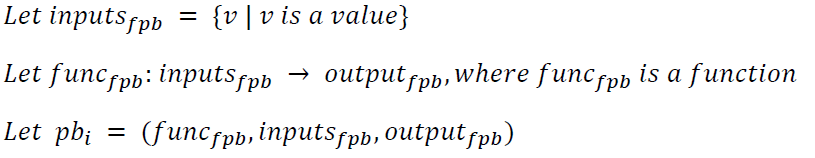
\includegraphics[scale=0.5]{Proof1-Part1.png} 
\end{center}

Firstly, the inputs for a program block is declared. The inputs are considerate as a set of values which can represent any possible value of any type. Then, a function is declared, it accepts some inputs and return as result an output. This function has to be considerate as the implementation of a program block. At the end, a program block is created as triple composed of function, inputs and output. 

\noindent
\newline
\textbf{4.3.1.2. Declaration of all program blocks}
\begin{center}
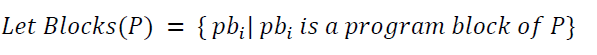
\includegraphics[scale=0.5]{Proof1-Part2.png} 
\end{center}

After the declaration of a program block, the entire program is defined by Blocks(P). The logic behind is that a program is composed of several program blocks that can be considerate as a set of program blocks. 

\noindent
\newpage
\textbf{4.3.1.3. Declaration of a test}
\begin{center}
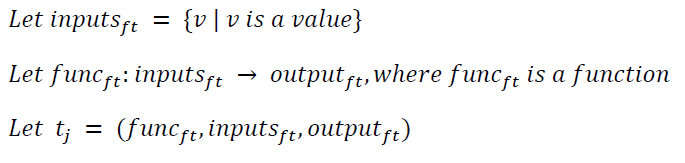
\includegraphics[scale=0.5]{Proof1-Part3.png} 
\end{center}

The declaration of a test is similar to a program block. The big difference is that the output of a test and of a program block can be different. For representing a test $t_j$, a triple is used and it is composed of function which is the implementation of a test, inputs and outputs.  

\noindent
\newline
\textbf{4.3.1.4. Declaration of all test sets for P}
\begin{center}
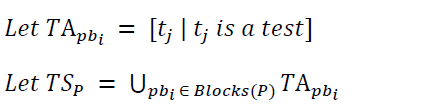
\includegraphics[scale=0.5]{Proof1-Part4.png} 
\end{center}

Then, a declaration of all tests performed on the program P is done by firstly considerate an array of tests which is a simple matrix (1xn). Then a set of all tests is declared by performing the union of all arrays composed of several tests. 

\noindent
\newline
\textbf{4.3.1.5. Show the validity and success of a test on a program block}
\begin{center}
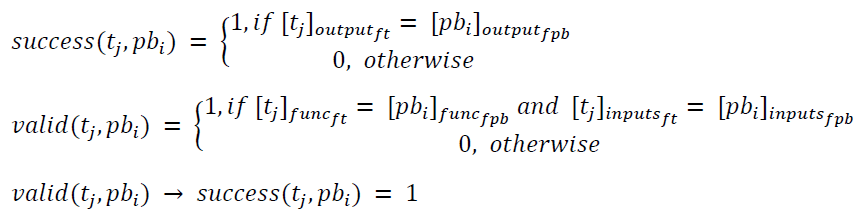
\includegraphics[scale=0.5]{Proof1-Part5.png} 
\end{center}

Now, in order to show the correctness of a program block, a test is applied to a program block by using the success($t_j$,$pb_i$) variable. 
\newline
success($t_j$,$pb_i$) accept two inputs, a test and a program block and provide as result 1 when the output of test is equal to output of program block, otherwise 0. If the result is 1 then a test is successful, otherwise 0 which is a failure. 
\newline                                                                                                                                                   As, not all tests can be performed on a program block because some are dedicated to other program blocks, a test has to be validated in order to understand, if it is the right test to perform. This is realize by valid($t_j$,$pb_i$) which accepts a test and a program block as inputs and provide a result which indicates if a test can be applied to a program block. The result is 1 when the inputs and the implementation of a program block and of a test are similar, in other case 0. %If, the result of validation is 1 then a test can be performed and it must be successful.
\noindent
\newline\newline
\textbf{4.3.1.6. demonstration that the whole program is correct}
\begin{center}
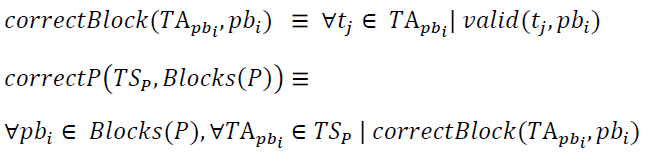
\includegraphics[scale=0.5]{Proof1-Part6.png} 
\end{center}

The final step of this demonstration consists to demonstrate if the whole program is correct. For explaining this part, a bottom up approach is used. 
\newline
For testing the entire program all the tests have to be performed on each program block. So, a set of all subsets of tests dedicated to each program block is taken. Then, each test of theses subsets is applied to a program block which are first validated and then tested. 
\subsubsection{Second demonstration}

\noindent
\newline\newline
\textbf{4.3.2.1. Declaration of pre and post conditions}
\begin{center}
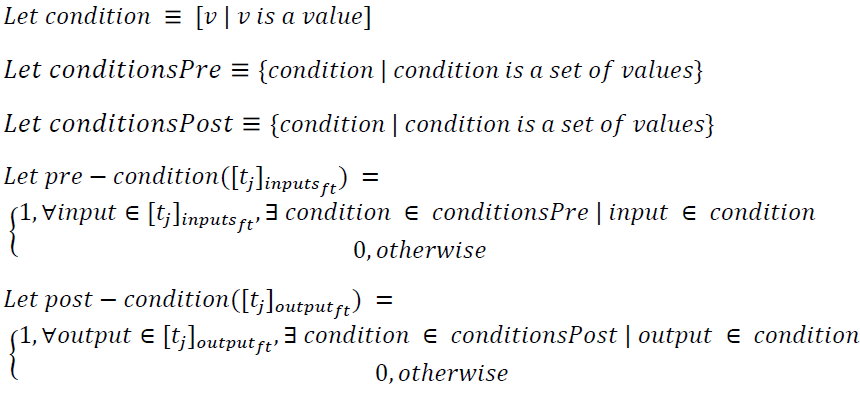
\includegraphics[scale=0.4]{Proof2-Part1.png} 
\end{center}

Firstly, define a ``condition" as an array of values which can be of any values and any types. Then, the ``conditionsPre" and ``conditionsPost" which represent the pre-conditions and post-conditions are defined, each by a set of ``condition".  
\newline
Next, ``pre-condition($[t_{j}]_{inputs_{ft}}$)" and ``post-condition($[t_{j}]_{outputs_{ft}}$)" functions are used for evaluating the inputs and outputs of a test with respect to ``conditionsPre" and ``conditionsPost". The ``pre-condition($[t_{j}]_{inputs_{ft}}$)" return 1 as result when for each input in inputs, it exists at least one condition in conditionsPre where the input belongs to condition, 0 otherwise. 
\newline
The same is done with ``post-condition($[t_{j}]_{outputs_{ft}}$)" but instead of inputs, outputs are used and are evaluated based on conditionsPost.  

\noindent
\newline
\textbf{4.3.2.2. Definition of all requirements}
\begin{center}
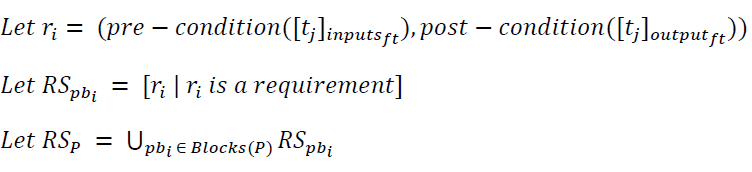
\includegraphics[scale=0.5]{Proof2-Part2.png} 
\end{center}

Each requirement is composed of two functions which allow to validate the inputs and the outputs of a test. Then, for each program block, it exists an array of requirements ${RS}_{{pb}_{i}}$ that have to be satisfied for the correctness of a program block. At the end, all the requirements are defined as a set of all requirements ${RS}_{{pb}_{i}}$. 

\noindent
\newpage
\textbf{4.3.2.3. Test satisfaction of a requirement}
\begin{center}
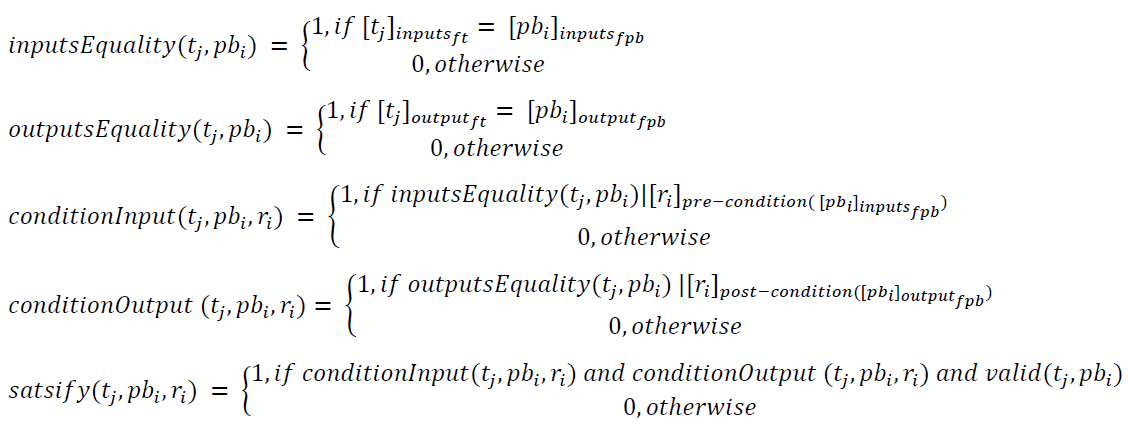
\includegraphics[scale=0.35]{Proof2-Part3.png} 
\end{center}

In this section, the satisfaction of a requirement is described by firstly looking at the equality of inputs and outputs between a test and a program block. For this purpose, two functions are declared, ``inputsEquality" and ``outputsEquality". ``inputsEquality" compare the inputs and ``outputsEquality" compare the outputs. 
\newline
Then, the inputs and outputs of a test and a program block have to be in requirement. For demonstrating that the inputs are in a requirement,first, the inputs of a test must be equal to inputs of a program block. Secondly, the inputs of a program block are evaluated based on ``pre-condition" function from the requirement. The same strategy is applied to outputs but instead of ``pre-condition", ``post-condition" is used. 
\newline
For testing the satisfaction of a requirement, ``satisfy" function is used and accept as inputs a test, a program block and a requirement. So, for satisfying a requirement the inputs and outputs of a program block and a test have to belong to the requirement and the test must be valid and successful. 


\noindent
\newline
\textbf{4.3.2.4. A specific requirement is satisfied for a program block}
\begin{center}
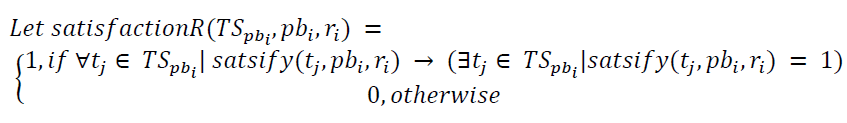
\includegraphics[scale=0.5]{Proof2-Part4.png} 
\end{center}

For demonstrating the satisfaction of a concrete requirement, the ``satisfy" function is performed on each test for showing if the requirement is satisfied or not. Then, between all the performed tests, it must exist one test where the ``satisfy" function return 1 and satisfy the requirement. 

\noindent
\newline
\textbf{4.3.2.5. All requirements are satisfied for a program block}
\begin{center}
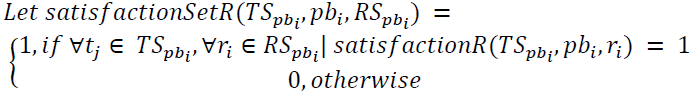
\includegraphics[scale=0.5]{Proof2-Part5.png} 
\end{center}

Then, all requirements have to be satisfied for a program block. For achieving this objective, ``satisfaction" function from previous section have to be reused on the whole array of tests and on the whole array of requirements for a program block. At the end, all the requirements for a particular program block have to be satisfied. 

\noindent
\newline
\textbf{4.3.2.6. All requirements are satisfied for a program}
\begin{center}
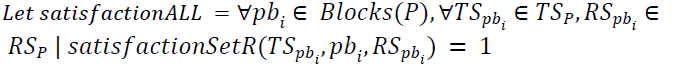
\includegraphics[scale=0.5]{Proof2-Part6.png} 
\end{center}

At the end, for proving that the program is correct from the behavior point of view. All the requirements have to be satisfied. So, all the tests performed on each program block must be successful and all the requirements defined for each program block have to be satisfied. 

\subsubsection{How the demonstrations can be applied to check the correctness of a program}
For looking for the correctness of a program based on unit testing. A program must be already developed and which is correct from the syntactical point of view. Moreover, the created program must be composed of functions or of parts of codes that can be individually separated from the entire program. The reason is that for the demonstrations, a program block is considerate as a function which accept inputs and produce an output.
\newline 
The question is how the demonstrations can be applied to the Jobs Observer web application?
\newline                                                         
Firstly, the Jobs Observer web application is developed in a way that it is composed only with the functions or individual parts of codes that can be separately tested. For showing how the demonstrations can be applied, only views.py module will be used because the entire program is too big for the demonstration. 

\noindent
\newline
\textbf{4.3.3.1. Application of first demonstration based on views.py module}

Let's considerate this views.py as a subprogram of Jobs Observer which will be our program to test. At beginning, this program has to be divided into blocks which consist of functions that accept a request as input and provide a Http response as output. 
\newline                                                                                                                                                   
Then, different test cases must be created for each program block to test. Each block can have one or more test cases which will be considerate as an array of tests. All these array of tests are considerated as a set of tests for testing the entire program.  
\newline                                                                                                                                     
When all tests are created, all tests of all arrays are applied for testing all program blocks. All the tests in each array will be passed and check for the validity for showing if a test is the right test for testing the program block. If, the test is valid then it is applied to the program block and the result of outputs are compared. If, the outputs are the same, in our case is a Http response, then the test is considerate as success, otherwise it fails. \newline
In the demonstration, if one test fails then the entire program will be considerate as incorrect. So, all the functions of views.py module must be correct. Thus, the entire program will be considerate correct. So, based on this demonstration, we showed how a part of a Jobs Observer can be tested for execution correctness.
\newline
For showing that the entire Jobs Observer is correct, all the subprograms(modules) must be correct executed. 

\noindent
\newpage
\textbf{4.3.3.2. Application of second demonstration}
So, for performing a second demonstration, the requirements have to be defined for views.py module, as an example each function return a HTTP response to the right HTML page.
\newline
When, all the requirements are created, the same tests can be performed on the views.py module as for the first demonstration, but before to perform a test, the satisfaction of requirement have to be applied on inputs and outputs. 
\newline
Then, during the process of testing all the tests, the requirements are also evaluated for the satisfaction for each program block. It means that for each program block all the requirements, dedicated to this program block, have to be satisfied. If, for each program block all the requirements are satisfied and all the tests are successfully passed, as example all the tests on a program block return a HTTP response to the right HTML page, then the program block behaves as expected. 
\newline
If, all program blocks satisfy all the requirements, then the behavior of the whole program is correct. 
                                                                                                                                          
\subsection{Assessment}
In this section, the comparison of scientific deliverables with respect with the requirements previously defined is described. 

\subsubsection{Evaluation of demonstrations}
The first requirement for the first demonstration is satisfied because the created demonstration demonstrate the correctness of a program by using the unit testing. Additionally, the demonstration demonstrates how the correctness of a program can be achieve if it is composed of several subprograms. 
\newline
The second requirement is also satisfied because the second demonstration demonstrates the correctness of a program not only from the execution point of view but also from the requirements point of view. 
\newline
The third requirement and the fourth requirements are also successfully achieved because the both demonstrations use the logical reasoning. So, the two demonstrations are based on mathematical demonstration by using step by step approach for arriving to a conclusion. Moreover, they are based on Natural Deduction. 
\newline
The fifth requirement is also achieved. Before starting to develop demonstrations, some notations are set and explained for improving the understandability. 

\subsubsection{Explanation on how the demonstrations can be use on Jobs Observer}
The first requirement for this part is met because the demonstrations can be applied to the real-world problem which was been shown with the Jobs Observer views.py module. For satisfying the demonstrations some assumptions have to be define and the program to test must be conform to these assumptions in order to make the demonstrations work. 
\newline
The second requirement is partially satisfied. The second requirement consists to provide an explanation which is consistent with respect to demonstrations, so that each part explained can be find in the demonstrations. The reason why this requirement is partially satisfied is that some parts for the program have to be assumed, as example the requirements for the program or when the views.py module in Jobs Observer is correct, we considerate all other program blocks also correct for demonstrating that the whole Jobs observer is correct.  


\section{Project technical deliverables}

\label{sec-production}
\subsection{Requirements}

In this Bachelor Semester Project, there are several requirements that must be satisfied for the technical part. These requirements are divided into two parts: front-end and back-end. For each part, functional and non-functional requirements will be discussed. 
\subsubsection{Front-end}
\noindent
\newline\newline
\textbf{5.1.1.1. Front-end functional requirements}
\newline

In this section, we will see the most important functionalities that the front-end must satisfies. The front-end consists to design a GUI that allows the interaction between web-server and end-users. 
\begin{itemize}
	\item FR1: Graphical User Interface should be created by using static pages in order to obtain a first visual representation of the web application. These static pages must have some basic elements of a webpage allowing simple interactions.

\item FR2: The GUI static pages must have the possibility to display statistics by using buttons in order to allow the execution of back-end python script. 
\end{itemize}
	
\noindent
\newline\newline
\textbf{5.1.1.2. Front-end non-functional requirements}
\newline

\begin{itemize}
\item NFR1: Friendly interface. The GUI should be easy to use without spending a lot of time for learning. Moreover, the user interface has to be intuitive so that the user can expect in advance the result produced by taking an action on an element of web page. Moreover, the basic elements of a webpage must be found in the right places. 
\newline
\item NFR2: Readability: The font-size of components of GUI must be easily visualize so that the information transmit by a GUI element can be easily understand by the user. Moreover, each static page must be not overload with the data in order to avoid the misunderstanding and confusion. 
\end{itemize}

\newpage
\subsubsection{Back-end}

\noindent
\newline\newline
\textbf{5.1.2.1. Back-end functional requirements}
\newline

In this section, the most important functionalities that the back-end must satisfies are described. The back-end part consists to develop a web-application which is deployed on an AWS server. 
\newline

\begin{itemize}
	\item FR1: The development of web-sever must be realized by using Django framework which is written in Python and the compatibility between Django web-server and AWS server has to be ensured. 
\newline

\item FR2: The old database from the existed software has to be used in the Jobs Observer. As the database file is too big, it should be imported from an external source such Dropbox from where it will be downloaded and reused. 
\newline
As, the old database is designed by using peewee library, which is a local database, Jobs Observer has to reuse the codes from the existed software for making the database working. 
\newline

\item FR3: Operations. All the operations for statistics creation have to be imported to the Jobs Observer in order to apply them on GUI buttons. When a statistic is requested by clicking on front-end button, some of operations have to be used in the right order for producing a statistic. 
\newline
Moreover, the operations to use must be operational and provide the right results. Additionally, the creation of all statistics must be made in Django views.py module. 
\newline

\item FR4: The back-end must be connected in a certain way to the front-end in order to execute the operations requested from the front-end and display the result of the operations at front-end. 
\end{itemize}

\noindent
\newline\newline
\textbf{5.1.2.2. Back-end non-functional requirements}
\newline

\begin{itemize}
\item NFR1: Maintainability. The development of web-server must be done in a way that it can be maintainable after the end of the project. For ensuring this requirement, a structural approach has to be used, some comments have to be written for the understandability of the program. The right naming must be used for operations and variables. 
\newline

\item NFR2: Operationality. The web-sever must be operational after the development for allowing the execution of different statistics and to be able to provide some firsts results. 
\newline

\item NFR3: Compatibility. The created web-server must be compatible with AWS for allowing Jobs Observer to run continuously and non-locally. 
\end{itemize}

\subsection{Design}
\subsubsection{Project creation}
The first step for designing the project, is the creation of Jobs Observer on AWS. The creation is realized by using a development tool called CodeStar which allows the creation of simple project and also more complex project such as a web-application.
\newline
For creating the project, a Django framework is used, based on the Python language. Additionally, the project source code of the project can be found on github which allows to perform an incremental development. 
 
\subsubsection{Graphical User Interface}
Before passing to the development part of web application, we will focus on the Graphical User Interface design. 
\newline
The first part consists to create a mockup by using an external online tool for creation of web sites. The creation of mockup is started by defining the structure of each page such as the locations of buttons, images and content. Then, the order in which these pages can be accessed is imposed in order to ensure the logical passage between one page to another. 
\newline
There are in total four pages that are designed such home, about software, plots and statistic which can be considerate as the basis for the future development. 
\newline
Then, the designed mockup was been used for created HTML pages for representing the content and a structure. CSS language is used for improving the visual representation of HTML pages. 

\subsubsection{Django structure}
Django framework has a defined structure which is used for development of web application. This structure is divided into two folders which allows the development and configuration of a web application. The first folder, called ``ec2django" is used for the configuration. The second folder, called ``helloworld" is used for the development of application.

\noindent
\newline\newline
\textbf{5.2.3.1. Configuration}
\newline
The ``ec2django" folder is used for the configuration and contains four python modules such init, settings, urls and wsgi. The settings.py module is the most important and is the only one module in which some modification are performed. It allows to setup application parameters such as path to HTML static pages, type and location of database and the middleware.
\newline
During the development, this module is used for indicating the location of CSS files that are reused by HTML files for design. Moreover, it is used for performing some changes in middleware classes for allowing a local execution. 

\noindent
\newline\newline
\textbf{5.2.3.2. Development}
\newline

The ``helloworld" folder is used for the development of a web application (Notice: the ``helloworld" name is the default name of application). As previously, this folder contains some modules such as init, admin, apps, models, views and urls. For the explanations, we will focus only on the last three modules.

\noindent
\newline\newline
\textbf{5.2.3.2.1. models.py}
\newline\newline
This module is used for creation of database and declaration of database structure. As, we have already an existed database from the existed local software, this old database is reused for fetched the available jobs. Moreover, the oldest database was been created by using peewee package and the structure of database was been previously defined. So, the existed code is reused.  
\newline
Unfortunately, the existed database is too big (around 1.2GB) and can not be used directly from the repository. So, this database is manually stored on a cloud server, called dropbox. 
\newline
When this module is executed, the stored database file is download to an empty database file which is then used as the principal database. 

\noindent
\newline\newline
\textbf{5.2.3.2.2. views.py}
\newline\newline
This module is used for processing the requests from the GUI and allowing the interaction between the GUI and users. 
\newline
This module is composed of several functions, called ``views", which accept a request and return a HTTP response composed of a request and a HTML page to display. As, we have design previously different HTML pages for our web application, these functions are used for indicating the right HTML page to display. 
Additionally, it is possible to perform some additional operations in between that allow the creation of different statistics. Theses created statistics are themselves the HTML pages and can be returned in HTTP response. 

\noindent
\newline\newline
\textbf{5.2.3.2.3. urls.py}
\newline\newline
This module is used for indicating the right urls for each view function in views.py module. This module is composed of a list of urls which are associated to each view function in views.py module. So, after the execution of a view function, an url is requested for displaying a HTML page. 

\noindent
\newline\newline
\textbf{5.2.3.2.4. stats.py}
\newline\newline
This module is one of the most important modules because it is used for creating different statistics based on available jobs in Computer Science. This module contains many functions that can be used for statistics creation. 
\newline
Usually for creating a statistic, a dataframe is firstly created and is used for creation of a plot or a table which represent a statistic. For creating the statistics, this module uses previously imported database for retrieving the data.   

\subsection{Production}
In this section, the description of the deliverable concrete production will be explained. For this section, the deliverable is divided into two parts, front-end and back-end deliverable. Notice that this deliverable is only a prototype and represent the basis for future development.
                                 
\subsubsection{Front-end deliverable}
Front-end deliverable is a Graphical User Interface view which is composed of several HTML pages that are used for the interaction with the web-application. In total the front-end deliverable contains four HTML pages such as ``Home", ``About Software",``Plots" and ``Statistic". 

\noindent
\newline\newline
\textbf{5.3.1.1 Home page (Figure 1)}
\newline\newline
The ``Home" page is the first HTML page which is shown to the user when he accessed the web application. The purpose of this page is to show what kind of statistics are offered by the web application and to redirect a user to other pages where he will be able to find the descriptions of possible statistics or some general information about the software.                                                                                   
\newline
The ``Home" page is separate into three parts such top, middle and bottom. The top of the page is a menu bar which is composed of a ``BiCS" image on the left and some buttons to the right. There are six buttons to the right such ``Home", ``About Software", ``Plots",``Tables",``Text" and ``About us" which are use for redirect the user to other HTML pages. At the moment, there are only three first buttons which are operational.                                                                                                                                            
\newline
The middle of the page is composed of four circles which are the clickable buttons. The biggest button contains the name and a logo of web application and is used for redirect the user to an ``About Software" page. The other three small buttons include images which show what kind of statistics are possible. Based on the title inside of images, the user is redirected to the right pages.                                                                   
\newline
The bottom of the page is reserved for additional information such as contact, Help\&FAQ and Social Media but not yet completely finished.  
\newline      
For the next pages the top and bottom of each page is the same as in the ``Home" page.                                                   
     
\noindent
\newline\newline
\textbf{5.3.1.2 About Software page (Figure 2)}
\newline\newline
The purpose of this page is to provide a user with the general information about the software. This page provides three types of information. The first is an overview about the software where the purpose of web application is described. The second describes what are the possible statistics and the third describes how the software works. Each description is placed into a white box label. 

\noindent
\newline\newline
\textbf{5.3.1.3 Plots page (Figure 3)}
\newline\newline
The purpose of this page is to provide a description of what kind of statistics are possible and to allow a user to choose a statistic to display. The description of each statistic can be found in a white box whihc is composed of a title (the name of statistic) followed by a small text of expected result. 
\newline
At the bottom of each white box, there are a button ``DISPLAY" which is used for displaying a statistic on another page. 
                                                                                                                                                      \newline                  
On this page, there are right now four description of statistics among which two are operational, ``Jobs Per Country" and ``Jobs Per Company".  These four descriptions are structured as follow, there are two statistic description per row and two per column.                   

\noindent
\newline\newline
\textbf{5.3.1.4 Statistic page (Figure 4)}
\newline\newline
This page appears after clicking on a ``DISPLAY" button from the ``Plots" page and is used for showing an interactive statistic. At the moment, only a statistic is displayed without any additional information. From the mockup point of view, the idea of this page is to display a window for a statistic and to add an additional information around.  

\subsubsection{Back-end deliverable}    
Back-end deliverable is a web application deployed on an AWS server. The web application is developed in Django and is composed of several modules. In this section, the concrete implementation of modules will be described such models.py, views.py, urls.py and stats.py and their relations. 

\noindent
\newline\newline
\textbf{5.3.2.1 models.py module}
\newline\newline
This module is used for the database creation and declaration of database structure.
\newline
At beginning, an existed database file, called ``jobs.db" is downloaded to the system from the Dropbox by using dropbox python package. This download is possible only, if it exists another database file inside the system. So, the ``jobs.db" database file from Dropbox is downloaded into an empty database file also called ``jobs.db" and this new file will be used as the new database. 
\newline
The reason to perform this download operation is that the existed database file from the previous software is too big and can't be store on github after the modification of the project.                                                  
\newline
Then, a structure for the database is declared for accessing the data and different tables of database. The database is composed of three types of table such ``Job", ``SearchQuery" and ``Token". 
\newline
``Job" table is composed of several attributes such id, county, company, etc. ``SearchQuery" table is composed of a term and a place which indicate the location. ``Token" is composed of jobs, values and order which are used for indicating the number of available jobs. 

\noindent
\newline\newline
\textbf{5.3.2.2 stats.py module}
\newline\newline
This module can be found in ``modules" folder. This module is imported from the existed software and is used for creating different types of statistics.
\newline
It provides three types of statistics: tables, plots and text which should be only created as HTML pages. In this module some changes are performed compare to initial version in order to allow the correct execution on the server. 
\newline
The first change consists to change all the paths to more common paths. Another, change consists to remove the read Excel sheet with all keywords because AWS server doesn't allow to load the Excel sheet as a dataframe locally and externally. There exists a solution for this problem which can be to create a new database externally and load the data from the Excel sheet into it.  

\noindent
\newline\newline
\textbf{5.3.2.3 views.py module}
\newline\newline
This module is used for interacting between the front-end and back-end which can be accessed from the ``helloworld" folder. It is composed of different functions called ``views" that accept a request and return a HTTP response to an HTML page. In this module there are three functions: get, change\_view and statistics\_view. 
\newline                                                                                                                                       
The get function is used for showing the ``Home" page when a user accesses the Jobs Observer.
\newline
The change\_view function is used for returning a HTTP response for ``About Software" and ``Plots" pages. This function is executed when the request method is a GET request. This GET request is defined as a dictionary with one value inside which indicates the name of the button in the HTML page. So, for this function the names are ``aboutSoftware" and ``plots" which represent the names of buttons in HTML pages.    
\newline
The statistics\_view function is used for displaying statistics requested by the user from plots page. The principle of execution is the same as for the previous function but instead directly to return a HTTP response for an HTML page, some operations have to be performed in between for creating a statistic HTML page. 
\newline
At the end, a HTTP response for the created HTML page is returned. The operations performed are the operation from the stats.py module. Let's take an example. 
\newline
A user request for a statistic, called ``Jobs Per Country". This request will be sent to views.py module and will pass through all the functions. The value of GET request is ``displayPlot1" and if this value is true for a certain ``if" method such if request.method == 'GET' and ``displayPlot1" in request.GET then some operations from stats.py will create a statistic which is used for returning a HTTP response. 

\noindent
\newline\newline
\textbf{5.3.2.4 urls.py module}
\newline\newline
This module is the last module before displaying a HTML page. It is composed of a list of urls where each name of url is associated to a function from views.py module. 
\newline
As example, the url called ``AboutSoftware" is associated to change\_view function.  Notice that the url ``AboutSoftware" is not a full url but a part of url which is considerate as the continuation of the basic url s.t basic url $+$ ``AboutSoftware".

\noindent
\newline\newline
\textbf{5.3.2.4 Project on AWS}
\newline\newline
Jobs Observer web-application is already deployed on AWS. The deployment is realized by putting the project on github which is attached to the AWS server. 

\subsection{Assessment}
In this section, the satisfaction of technical deliverable with respect to the requirements are compared and evaluated. As previously, the front-end deliverable and back-end deliverable are evaluated based on requirements. 

\subsubsection{Front-end deliverable}
The front-end deliverable which is the GUI interface of our web application, satisfies all the functional requirements. The accomplishment of the first requirement can be seen on (Figure 1) which shows that the GUI contains some basic elements of a web page. Additionally, the created page is a static page and contains some buttons that allow the creation of statistics.                                         
\newline
The second requirement is also satisfied because the buttons for displaying statistics are connected to the python script and are operational. 
The front-end deliverable also satisfies all the non-functional requirements which consist to have a friendly interface and a good readability. For the first requirement, a simple interface is created for avoiding to a user to spend a lot of time for learning because based on the names of buttons and titles, he would be able to predict the result in advance.
\newline                                                                                                     
For the third requirement, the GUI interface doesn't overload the user with a lot of information which increase the readability. Additionally, the font-size is adequate because it allows to see all the names of elements and to read all the text sections. 


\subsubsection{Back-end deliverable}
In this section, a comparison between the back-end technical deliverable produced and the back-end requirements is realized. The objectives are to identify, if all the functional and non-functional requirements are satisfied. 

\noindent
\newline\newline
\textbf{5.4.2.1 Satisfaction of functional requirements}
\newline\newline
The first functional requirement is satisfied. It consists to use Django for creating the Jobs Observer and to ensure the compatibility of Jobs Observer application with the AWS server. The technical deliverable is based on Django framework and is already deployed on AWS server. Additionally, some of  operations and user interactions are available and can be performed. 
\newline
The second functional requirement is also satisfied. It consists to import the database and to reuse the same structure in Jobs Observer from the previous software.  Jobs Observer use the same structure for the imported database. The imported database isn't included directly to Jobs Observer but is downloaded from the external cloud server to the empty database file. 
\newline
The third functional requirement is partially satisfied because the Jobs Observer contains all operations from previous software but not all of them are operational and some more changes have to be performed for reaching the satisfaction of the whole requirement. Nevertheless, some operations are available and provide as results the created statistics. 
\newline
The fourth functional requirement is satisfied. Some operations at back-end can be call for execution from the GUI. As the result for each operation, a single statistic is displayed. 

\noindent
\newline\newline
\textbf{5.4.2.2 Satisfaction of non-functional requirement}
\newline\newline
The first non-functional requirement is partially satisfied. Indeed, it is difficult to evaluate if the Jobs Observer is maintainable. The Jobs Observer is not yet a final product and can be improve. For simplifying further development, a structural approach, a meaningful naming for operations and variables are used. 
\newline
The second and the third non-functional requirement are satisfied. From the back-end functional requirements, it is possible to conclude that the back-end of Jobs Observer is operational and compatible with the AWS server. 


\section*{Acknowledgment}
I would like to thank Prof. Nicolas Guelfi for being my Pat and guiding me during the entire project. Furthermore, I would like to thank him for providing me a project which has a lot of fields where I can learn and improve myself in the domain of software engineering. 


\section{Conclusion}
In this Bachelor Semester Project, a Jobs Observer web application is created by using Django framework and is deployed on an AWS server. The goal of Jobs Observer is to deliver statistics based on jobs in Computer Science companies and countries. During the project, the development of front-end and back-end is explained and the end results are provided. In terms of results, the biggest part of requirements fixed at beginning are satisfied which conclude that the Jobs Observer development is successfully achieved. 
\newline
\newline
During the project, the demonstrations of correctness of a program is designed for identifying if a program is correct in terms of execution and behaviors. For showing the usage of the demonstrations, an explanation on how they can be applied on Jobs Observer is provided. From this explanation, we can conclude that the demonstrations can be used on real world problems and can show the correctness of a program but just before the program to test has to satisfy some assumptions. 


% An example of a floating figure using the graphicx package.
% Note that \label must occur AFTER (or within) \caption.
% For figures, \caption should occur after the \includegraphics.
% Note that IEEEtran v1.7 and later has special internal code that
% is designed to preserve the operation of \label within \caption
% even when the captionsoff option is in effect. However, because
% of issues like this, it may be the safest practice to put all your
% \label just after \caption rather than within \caption{}.
%
% Reminder: the "draftcls" or "draftclsnofoot", not "draft", class
% option should be used if it is desired that the figures are to be
% displayed while in draft mode.
%
%\begin{figure}[!t]
%\centering
%\includegraphics[width=2.5in]{myfigure}
% where an .eps filename suffix will be assumed under latex, 
% and a .pdf suffix will be assumed for pdflatex; or what has been declared
% via \DeclareGraphicsExtensions.
%\caption{Simulation results for the network.}
%\label{fig_sim}
%\end{figure}

% Note that the IEEE typically puts floats only at the top, even when this
% results in a large percentage of a column being occupied by floats.


% An example of a double column floating figure using two subfigures.
% (The subfig.sty package must be loaded for this to work.)
% The subfigure \label commands are set within each subfloat command,
% and the \label for the overall figure must come after \caption.
% \hfil is used as a separator to get equal spacing.
% Watch out that the combined width of all the subfigures on a 
% line do not exceed the text width or a line break will occur.
%
%\begin{figure*}[!t]
%\centering
%\subfloat[Case I]{\includegraphics[width=2.5in]{box}%
%\label{fig_first_case}}
%\hfil
%\subfloat[Case II]{\includegraphics[width=2.5in]{box}%
%\label{fig_second_case}}
%\caption{Simulation results for the network.}
%\label{fig_sim}
%\end{figure*}
%
% Note that often IEEE papers with subfigures do not employ subfigure
% captions (using the optional argument to \subfloat[]), but instead will
% reference/describe all of them (a), (b), etc., within the main caption.
% Be aware that for subfig.sty to generate the (a), (b), etc., subfigure
% labels, the optional argument to \subfloat must be present. If a
% subcaption is not desired, just leave its contents blank,
% e.g., \subfloat[].


% An example of a floating table. Note that, for IEEE style tables, the
% \caption command should come BEFORE the table and, given that table
% captions serve much like titles, are usually capitalized except for words
% such as a, an, and, as, at, but, by, for, in, nor, of, on, or, the, to
% and up, which are usually not capitalized unless they are the first or
% last word of the caption. Table text will default to \footnotesize as
% the IEEE normally uses this smaller font for tables.
% The \label must come after \caption as always.
%
%\begin{table}[!t]
%% increase table row spacing, adjust to taste
%\renewcommand{\arraystretch}{1.3}
% if using array.sty, it might be a good idea to tweak the value of
% \extrarowheight as needed to properly center the text within the cells
%\caption{An Example of a Table}
%\label{table_example}
%\centering
%% Some packages, such as MDW tools, offer better commands for making tables
%% than the plain LaTeX2e tabular which is used here.
%\begin{tabular}{|c||c|}
%\hline
%One & Two\\
%\hline
%Three & Four\\
%\hline
%\end{tabular}
%\end{table}


% Note that the IEEE does not put floats in the very first column
% - or typically anywhere on the first page for that matter. Also,
% in-text middle ("here") positioning is typically not used, but it
% is allowed and encouraged for Computer Society conferences (but
% not Computer Society journals). Most IEEE journals/conferences use
% top floats exclusively. 
% Note that, LaTeX2e, unlike IEEE journals/conferences, places
% footnotes above bottom floats. This can be corrected via the
% \fnbelowfloat command of the stfloats package.

% trigger a \newpage just before the given reference
% number - used to balance the columns on the last page
% adjust value as needed - may need to be readjusted if
% the document is modified later
%\IEEEtriggeratref{8}
% The "triggered" command can be changed if desired:
%\IEEEtriggercmd{\enlargethispage{-5in}}

% references section

% can use a bibliography generated by BibTeX as a .bbl file
% BibTeX documentation can be easily obtained at:
% http://mirror.ctan.org/biblio/bibtex/contrib/doc/
% The IEEEtran BibTeX style support page is at:
% http://www.michaelshell.org/tex/ieeetran/bibtex/
%\bibliographystyle{IEEEtran}
% argument is your BibTeX string definitions and bibliography database(s)
%\bibliography{IEEEabrv,../bib/paper}
%
% <OR> manually copy in the resultant .bbl file
% set second argument of \begin to the number of references
% (used to reserve space for the reference number labels box)
\begin{thebibliography}{1}

\bibitem[1]{}
\newblock {Software Testing: Basics.” GeeksforGeeks, 30 Apr. 2019,}
\newblock {https://www.geeksforgeeks.org/software-testing-basics/}.

\bibitem[2]{}
\newblock {Verification vs Validation.” Software Testing Fundamentals, 3 Mar. 2018.}
\newblock {http://softwaretestingfundamentals.com/verification-vsvalidation/}.

\bibitem[3]{}
\newblock {Rouse, Margaret, et al. “What Is Software Engineering? - Definition from WhatIs.com.” WhatIs.com,}
\newblock {https://whatis.techtarget.com/definition/software-engineering}.

\bibitem[4]{}
\newblock {“Différence Entre Le Développeur Front-End Et Le Développeur Back-End ?” Alticreation, 28 Sept. 2018,}
\newblock {https://www.alticreation.com/difference-developpeur-front-end-et-developpeur-back-end/.}.

\bibitem[5]{}
\newblock {“Mathematical Proof.” Wikipedia, Wikimedia Foundation, 12 Dec. 2019,}
\newblock {https://en.wikipedia.org/wiki/Mathematical\_proof.}

\bibitem[6]{}
\newblock {“3. Natural Deduction for Propositional Logic.” 3. Natural Deduction for Propositional Logic - Logic and Proof 0.1 Documentation,}
\newblock {https://leanprover.github.io/logic\_and\_proof/natural\_deduction\_for\_propositional\_logic.html.}

\bibitem[7]{}
\newblock {“Unit Testing.” Software Testing Fundamentals, 3 Mar. 2018,}
\newblock {http://softwaretestingfundamentals.com/unit-testing/.}

\bibitem[8]{}
\newblock {“Unit Testing Tutorial: What Is, Types, Tools, EXAMPLE.” Guru99,}
\newblock {https://www.guru99.com/unit-testing-guide.html.}

\bibitem[9]{}
\newblock {“What Is Python?” Python For Beginners,}
\newblock {https://www.pythonforbeginners.com/learn-python/what-is-python/.}

\bibitem[10]{}
\newblock {“Programming Language.” Wikipedia, Wikimedia Foundation, 3 Dec. 2019,}
\newblock {https://en.wikipedia.org/wiki/Programming\_language\#Dynamic\_semantics}

\bibitem[11]{}
\newblock {“What Is Dynamic Binding?” Computer Hope, 26 Apr. 2017,}
\newblock {https://www.computerhope.com/jargon/d/dynamic-binding.htm}

\bibitem[12]{}
\newblock {“Chegg.com.” Definition of Logical Reasoning | Chegg.com,}
\newblock {https://www.chegg.com/homework-help/definitions/logical-reasoning-63}

\end{thebibliography}
\newpage 
\onecolumn
\section{Appendix}

\begin{figure}[hbt!]
  \centering
	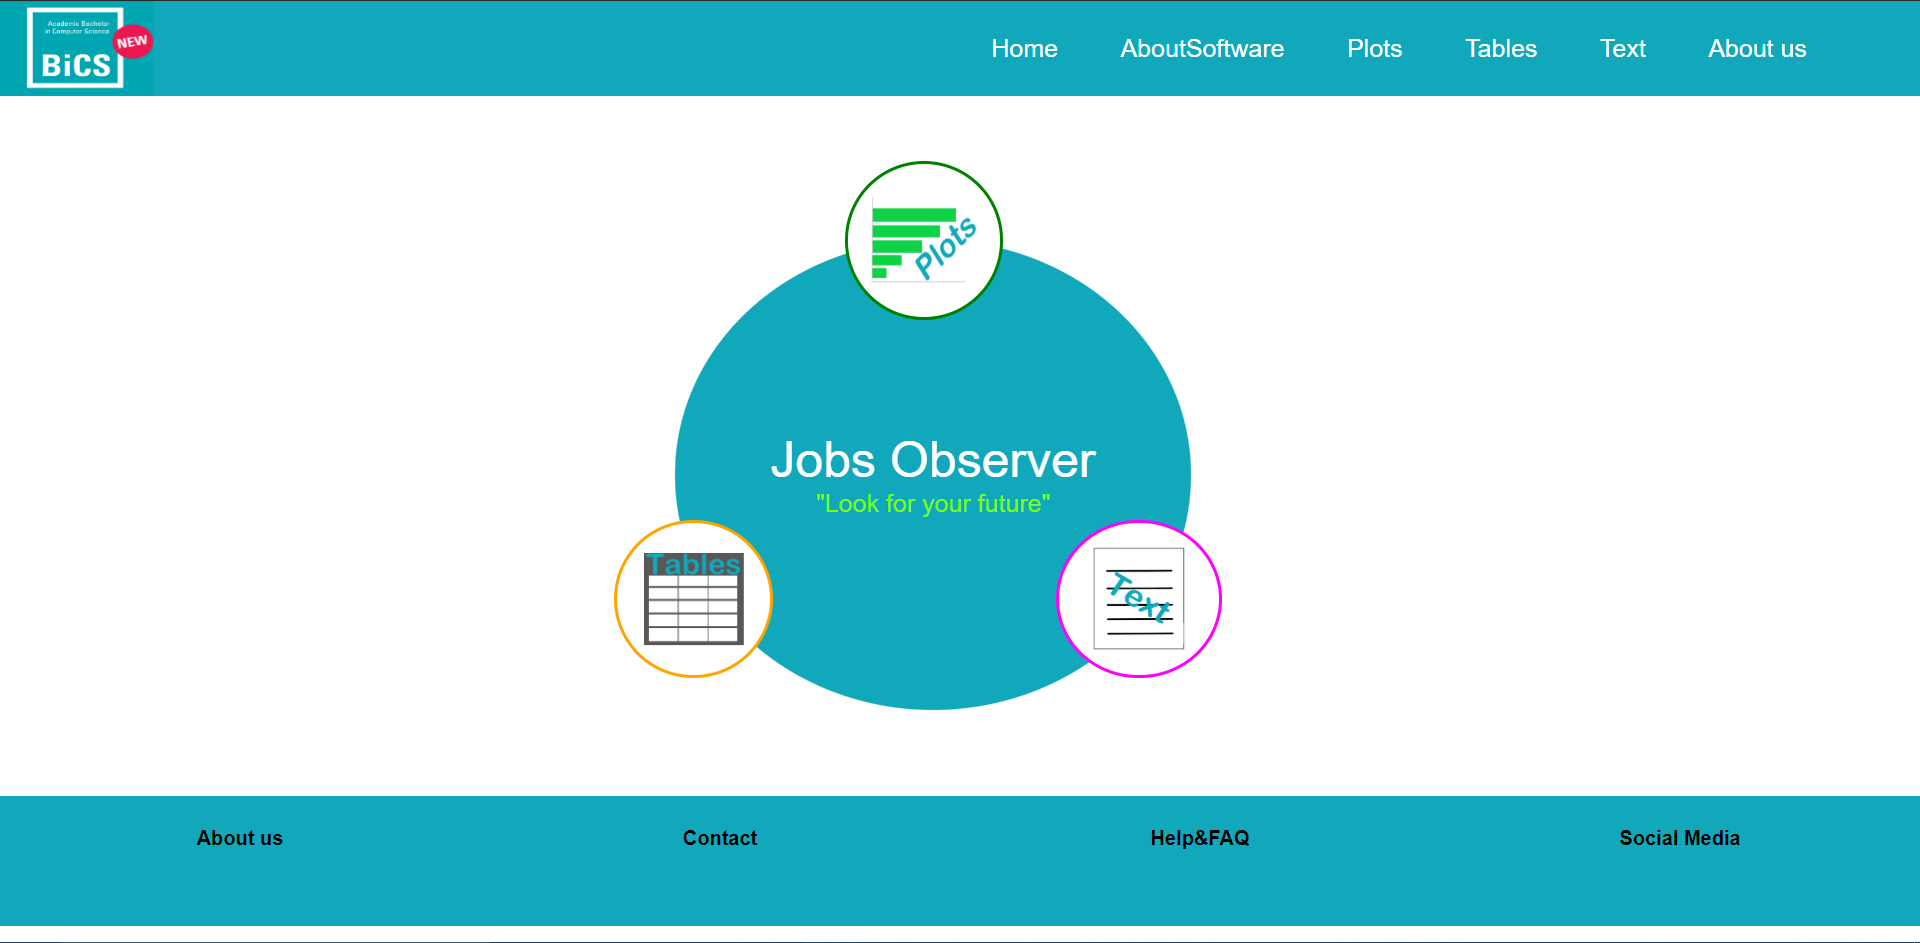
\includegraphics[scale=0.4]{home.png} 
	\caption{Home view of Jobs Observer web application}
\end{figure}

\begin{figure}[hbt!]
  \centering
	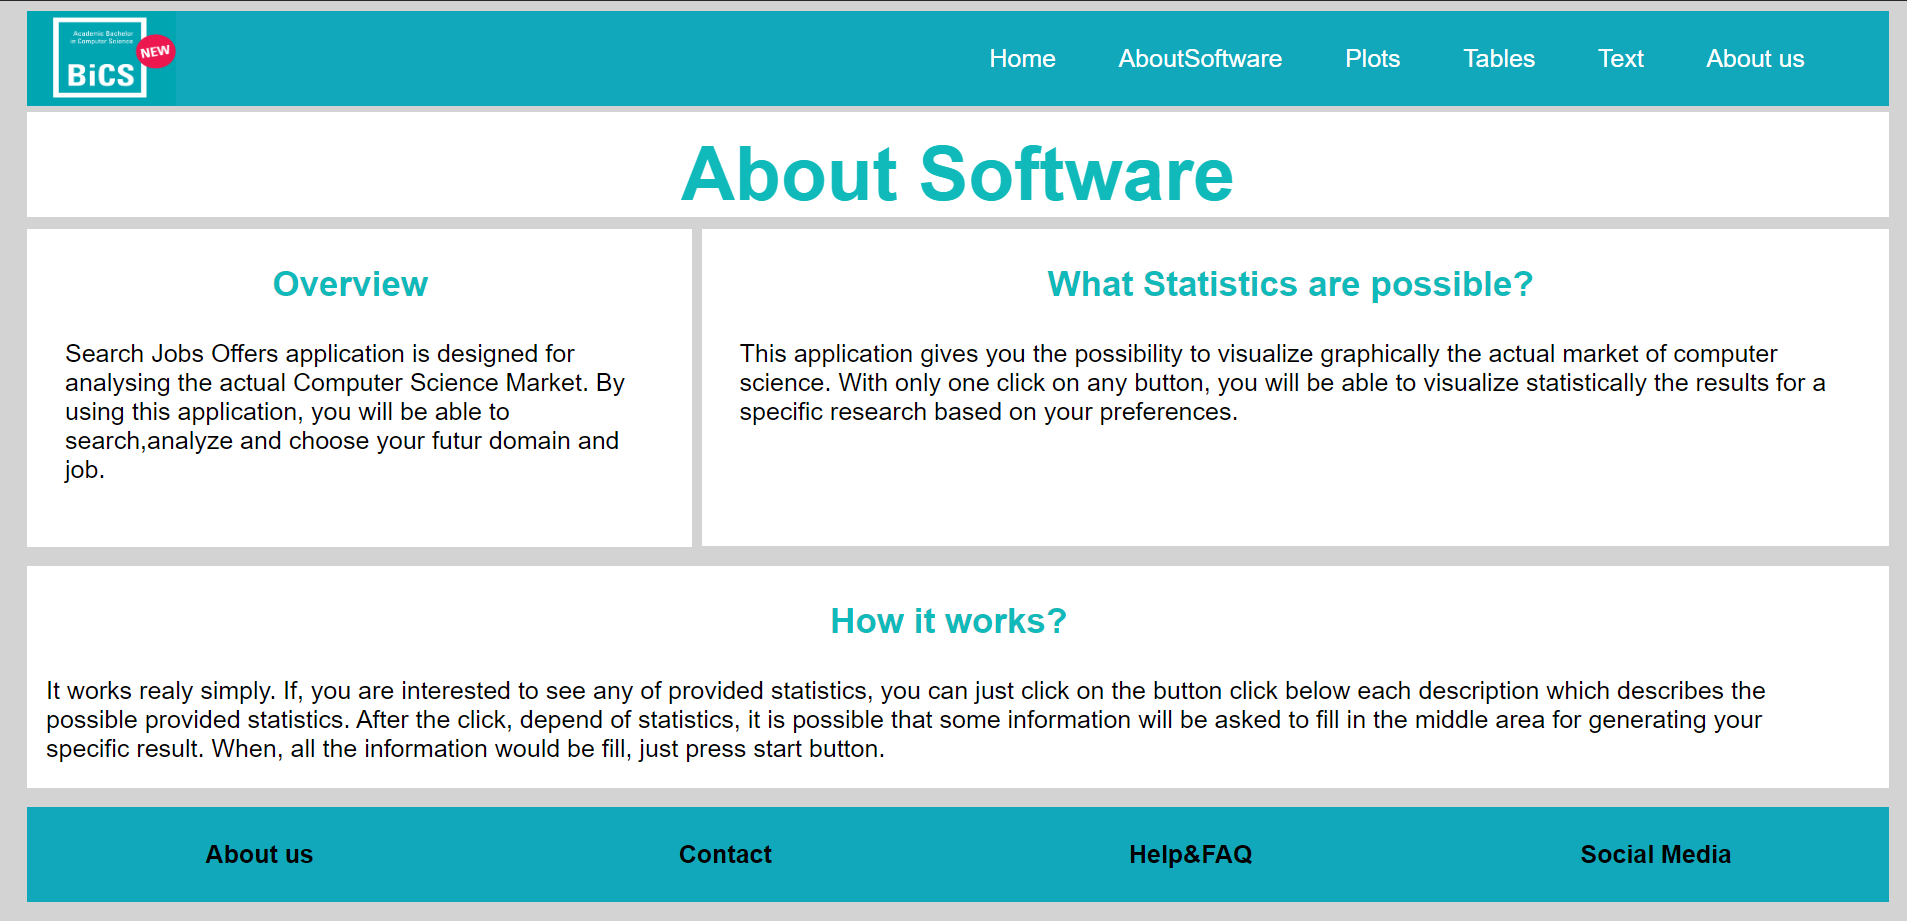
\includegraphics[scale=0.4]{aboutSoftware.png} 
	\caption{About Software page of Jobs Observer web application}
\end{figure}

\begin{figure}[hbt!]
  \centering
	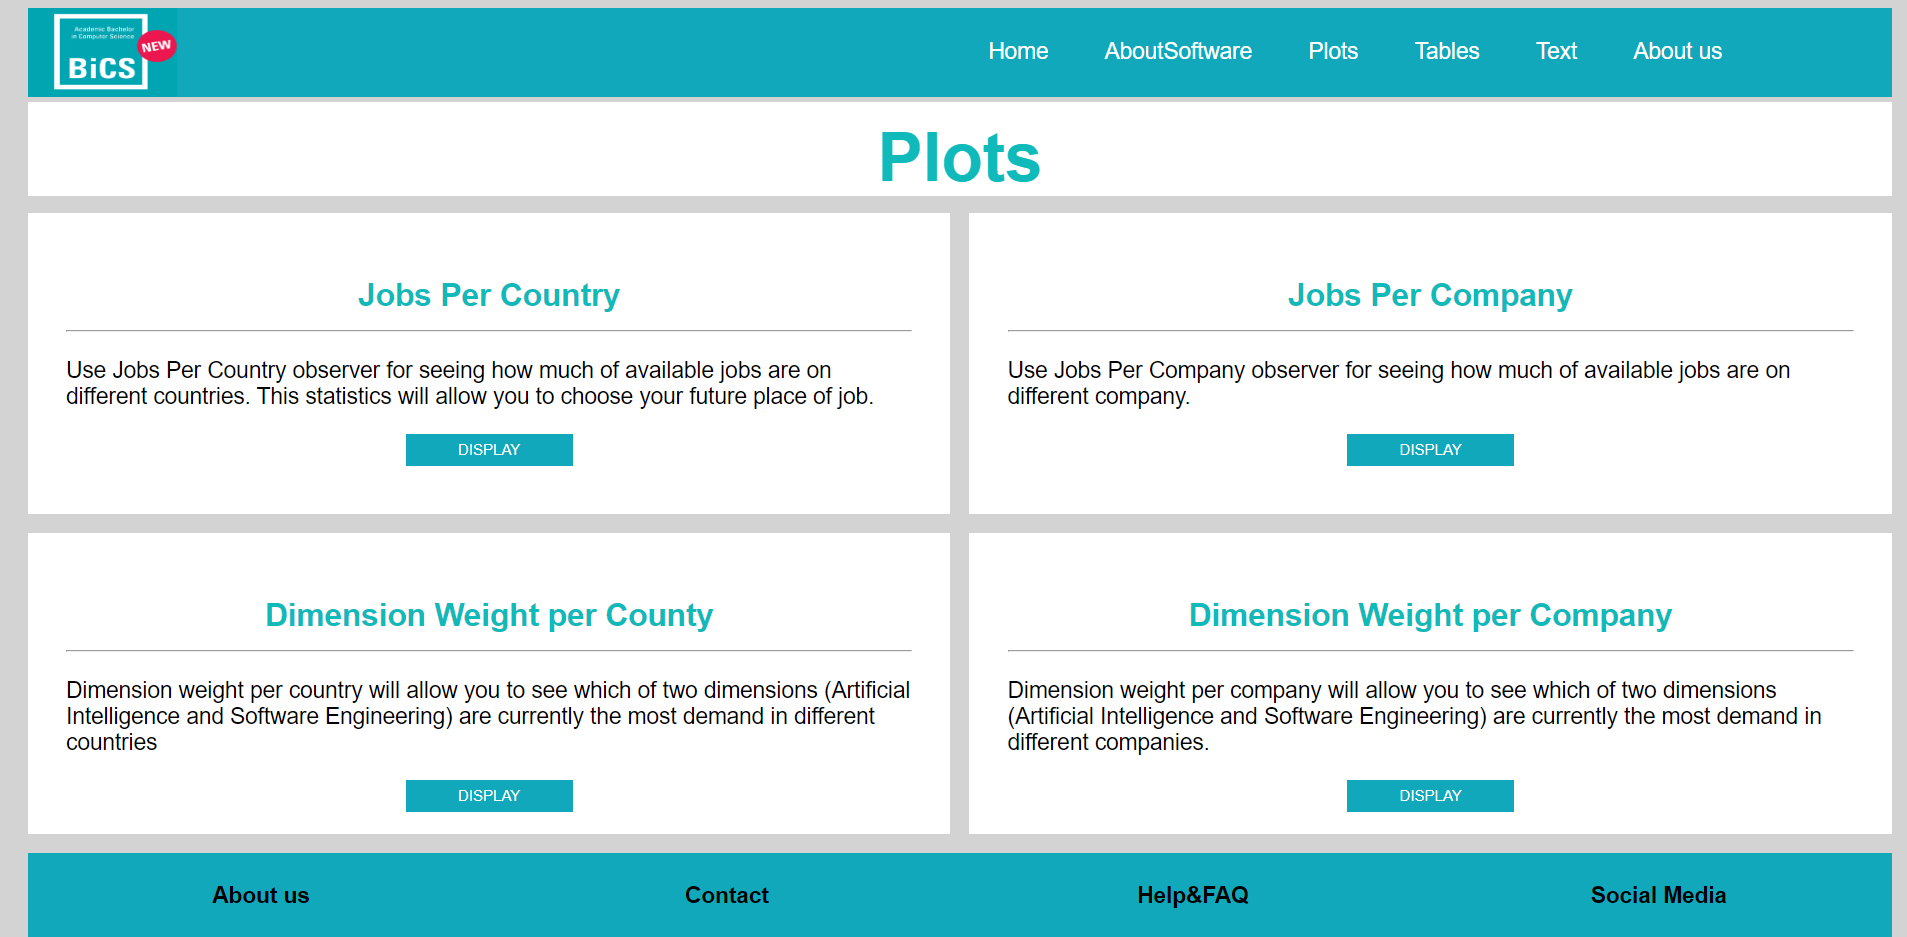
\includegraphics[scale=0.4]{plots.png} 
	\caption{Plots page of Jobs Observer web application}
\end{figure}

\begin{figure}[hbt!]
  \centering
	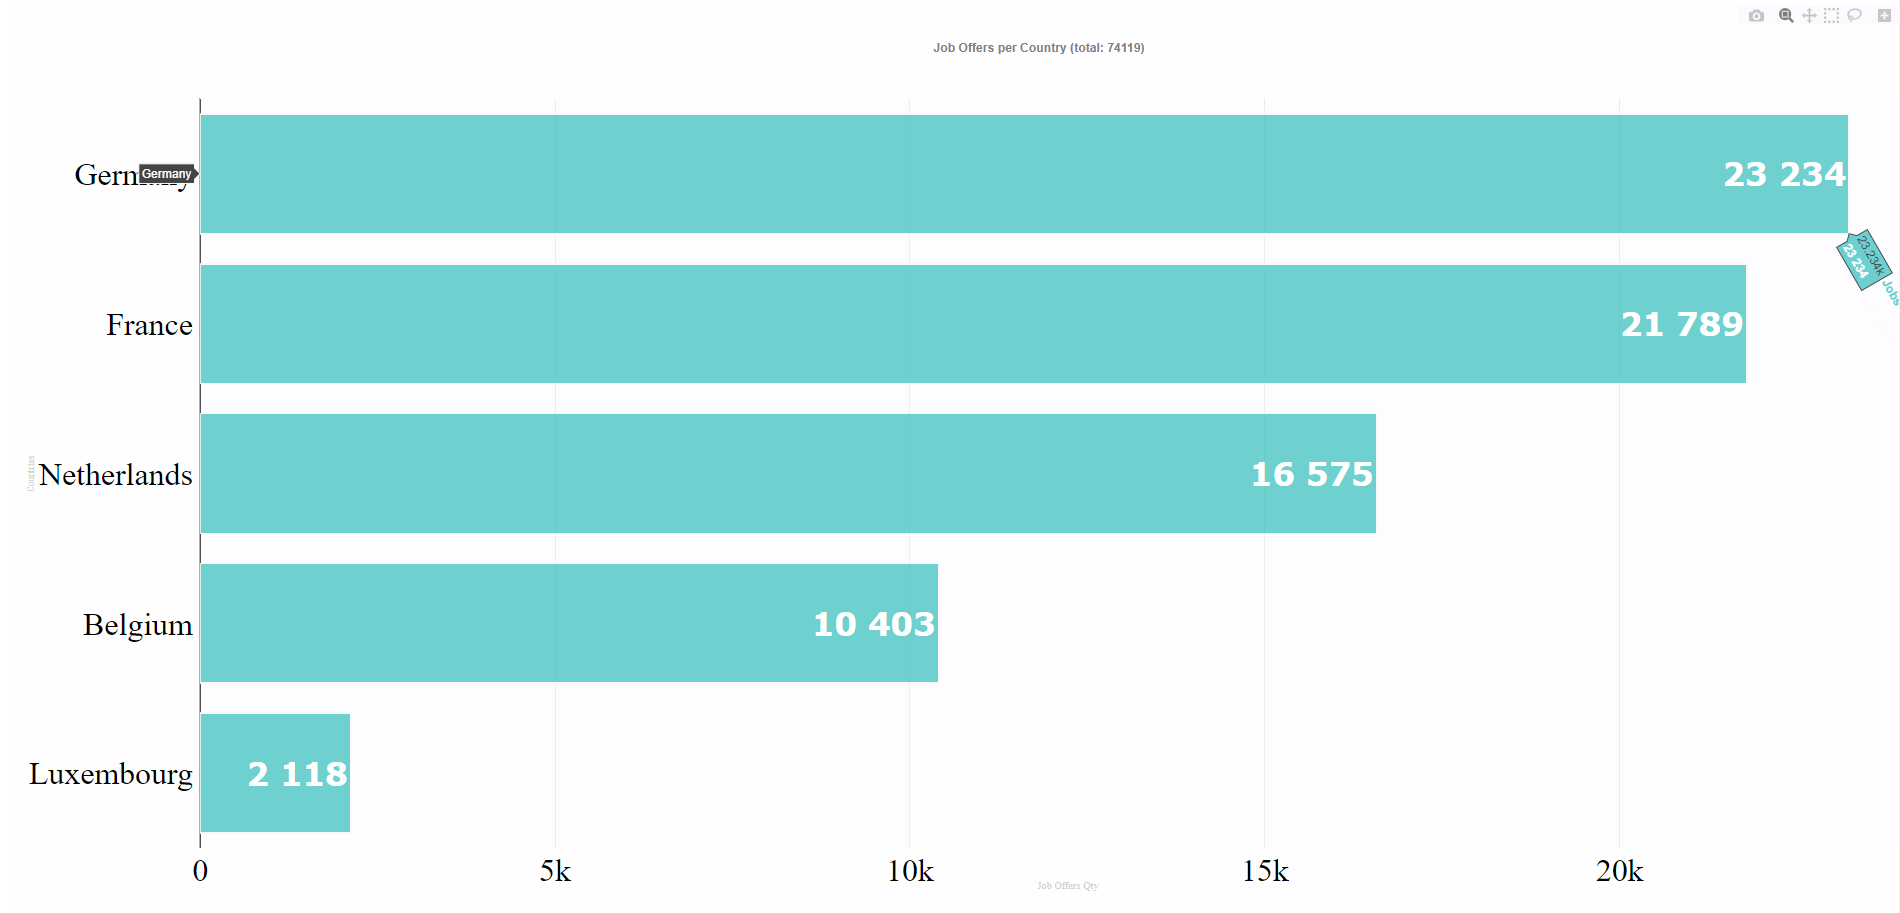
\includegraphics[scale=0.4]{statistic.png} 
	\caption{A statistic based on jobs per country}
\end{figure}

\end{document}

